\documentclass[11pt]{article}
\usepackage[margin=0.92in]{geometry}
\usepackage{amsmath,amssymb,amsthm,mathtools}
\usepackage{graphicx}
\usepackage{float}
\usepackage{xcolor}
\usepackage[hidelinks]{hyperref}
\usepackage{microtype}

\definecolor{accent}{HTML}{7A263A}
\definecolor{soft}{HTML}{FBEFF2}
\newtheorem{theorem}{Theorem}
\newtheorem{proposition}{Proposition}
\newtheorem{corollary}{Corollary}
\newcommand{\R}{\mathbb R}
\newcommand{\F}{\mathcal F}

\title{A sign error at critical structural damping:\\counterexample and corrected Mittag--Leffler kernels}
\author{Full correction to the $\mu=2$ formulas in arXiv:2212.10463v2}
\date{11 August 2026}

\begin{document}
\maketitle

\begin{center}
\fcolorbox{accent}{soft}{\parbox{0.91\linewidth}{
\textbf{Result.}  In the critical case $\mu=2$, two kernels used in
Theorems 6.3 and 6.4 of Faustino--Marques \cite{FM} have the wrong sign.
For every $1/2<\alpha<1$, their stated hyperbolic solution with nonzero
initial velocity fails the prescribed initial condition.  The error comes
from an incorrect recurrence for the Prabhakar function.  We prove the
correct recurrence, give a direct counterexample, and replace both affected
kernels.  The initial-displacement kernel is already correct.}}
\end{center}

\section{The printed identity}

The three-parameter Mittag--Leffler (Prabhakar) function is
\[
 E_{\alpha,\beta}^{\gamma}(w)
 =\sum_{k=0}^{\infty}
   \frac{(\gamma)_k}{k!}\frac{w^k}{\Gamma(\alpha k+\beta)}.
\]
The source's Lemma 4.3(iii) prints
\begin{equation}\label{eq:printed}
 \alpha E_{\alpha,\beta}^{2}(w)
 =E_{\alpha,\beta-1}(w)
 -(1+\alpha-\beta)E_{\alpha,\beta}(w).
\end{equation}
This identity is then used in the repeated-root formulas on pages 23, 25,
and 27.

\begin{figure}[H]
\centering
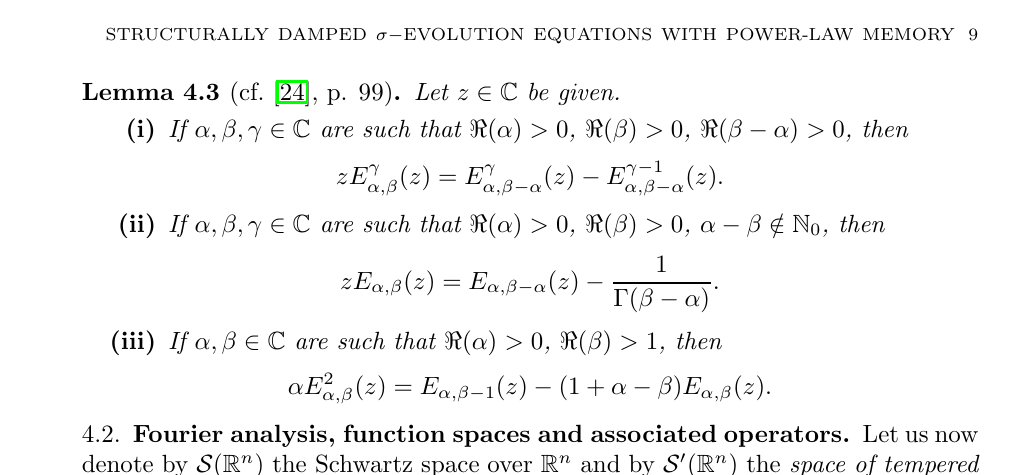
\includegraphics[width=0.84\linewidth]{figures/printed_false_identity_crop.png}
\caption{Lemma 4.3(iii) in arXiv:2212.10463v2, page 9.  The displayed
minus sign must be a plus sign.}
\end{figure}

There is already a zero-order check: at $w=0$, the left side of
\eqref{eq:printed} is $\alpha/\Gamma(\beta)$, whereas the printed right
side is $(2\beta-\alpha-2)/\Gamma(\beta)$.  These agree only in the
exceptional case $\beta=\alpha+1$.

\section{Correct recurrence}

\begin{theorem}[Prabhakar reduction]\label{thm:identity}
For $\alpha>0$ and $\beta\in\R$,
\begin{equation}\label{eq:correct}
 \boxed{\quad
 \alpha E_{\alpha,\beta}^{2}(w)
 =E_{\alpha,\beta-1}(w)
 +(1+\alpha-\beta)E_{\alpha,\beta}(w).
 \quad}
\end{equation}
Consequently, the difference ``printed minus correct'' is
\begin{equation}\label{eq:error}
 \frac{2(\beta-\alpha-1)}{\alpha}E_{\alpha,\beta}(w)
\end{equation}
after division by $\alpha$.
\end{theorem}

\begin{proof}
Since $(2)_k/k!=k+1$,
\[
 E_{\alpha,\beta}^{2}(w)
 =\sum_{k\ge0}(k+1)\frac{w^k}{\Gamma(\alpha k+\beta)}.
\]
On the other hand,
\[
 E_{\alpha,\beta-1}(w)
 =\sum_{k\ge0}(\alpha k+\beta-1)
   \frac{w^k}{\Gamma(\alpha k+\beta)}.
\]
Adding $(1+\alpha-\beta)E_{\alpha,\beta}(w)$ makes the coefficient
$\alpha(k+1)$ term by term, proving \eqref{eq:correct}.  Subtracting the
two alternatives gives \eqref{eq:error}.
\end{proof}

The same formula also follows by taking the divided-difference limit
\[
 \lim_{\lambda_+,\lambda_-\to1}
 \frac{\lambda_+E_{\alpha,\beta}(-\lambda_+z)
       -\lambda_-E_{\alpha,\beta}(-\lambda_-z)}
      {\lambda_+-\lambda_-}.
\]
Thus the apparent pole at the coalescing characteristic roots is
removable, and its value has the plus sign in \eqref{eq:correct}.

\section{Correct critical kernels}

Write $a=|\xi|^\sigma$ and $z=a t^\alpha$.  At $\mu=2$ the transformed
denominator is $(s^\alpha+a)^2$.  The source correctly obtains the
Prabhakar forms before replacing them by two-parameter functions:
\begin{align}
 \mathcal L^{-1}\!\left[\frac{s^{2\alpha-\beta}}
 {(s^\alpha+a)^2}\right]
 &=t^{\beta-1}E_{\alpha,\beta}^{2}(-z),\label{eq:Mlap}\\
 \mathcal L^{-1}\!\left[\frac{s^{2\alpha-2}}
 {(s^\alpha+a)^2}\right]
 &=tE_{\alpha,2}^{2}(-z).\label{eq:Jlap}
\end{align}
Indeed the general identity is
\[
 \mathcal L\{t^{\beta-1}E_{\alpha,\beta}^{2}(-at^\alpha)\}(s)
 =\frac{s^{2\alpha-\beta}}{(s^\alpha+a)^2}.
\]

\begin{proposition}[Replacement formulas]\label{prop:kernels}
In Notations 6.1--6.2 and equations (6.10), (6.18) of \cite{FM}, replace
the two critical multipliers by
\begin{align}
 m_{\mathrm{crit}}(t,\xi)
 &=\frac{t^{\beta-1}}{\alpha}
 \Big(E_{\alpha,\beta-1}(-z)
 +(1+\alpha-\beta)E_{\alpha,\beta}(-z)\Big),\label{eq:Mcorrect}\\
 j_{\mathrm{crit}}(t,\xi)
 &=\frac{t}{\alpha}
 \Big(E_{\alpha,1}(-z)
 +(\alpha-1)E_{\alpha,2}(-z)\Big).\label{eq:Jcorrect}
\end{align}
The critical initial-displacement multiplier remains
\begin{equation}\label{eq:Ncorrect}
 n_{\mathrm{crit}}(t,\xi)
 =E_{\alpha,1}(-z)+\frac{z}{\alpha}E_{\alpha,\alpha}(-z).
\end{equation}
With \eqref{eq:Mcorrect}--\eqref{eq:Ncorrect}, the Laplace-transformed
Cauchy equations and all prescribed initial data are satisfied.
\end{proposition}

\begin{proof}
Equations \eqref{eq:Mcorrect} and \eqref{eq:Jcorrect} follow from
\eqref{eq:Mlap}--\eqref{eq:Jlap} and Theorem \ref{thm:identity}, taking
$\beta$ and $2$, respectively.  For \eqref{eq:Ncorrect}, decompose
\[
 \frac{s^{2\alpha-1}+2as^{\alpha-1}}{(s^\alpha+a)^2}
 =\frac{s^{\alpha-1}}{s^\alpha+a}
  +\frac{a s^{\alpha-1}}{(s^\alpha+a)^2}.
\]
Its inverse is
$E_{\alpha,1}(-z)+zE_{\alpha,\alpha+1}^{2}(-z)$, and
\eqref{eq:correct} with $\beta=\alpha+1$ gives
$E_{\alpha,\alpha+1}^{2}=E_{\alpha,\alpha}/\alpha$.
The Laplace transforms are therefore exactly the rational multipliers
derived from the Cauchy equations.
\end{proof}

\begin{figure}[H]
\centering
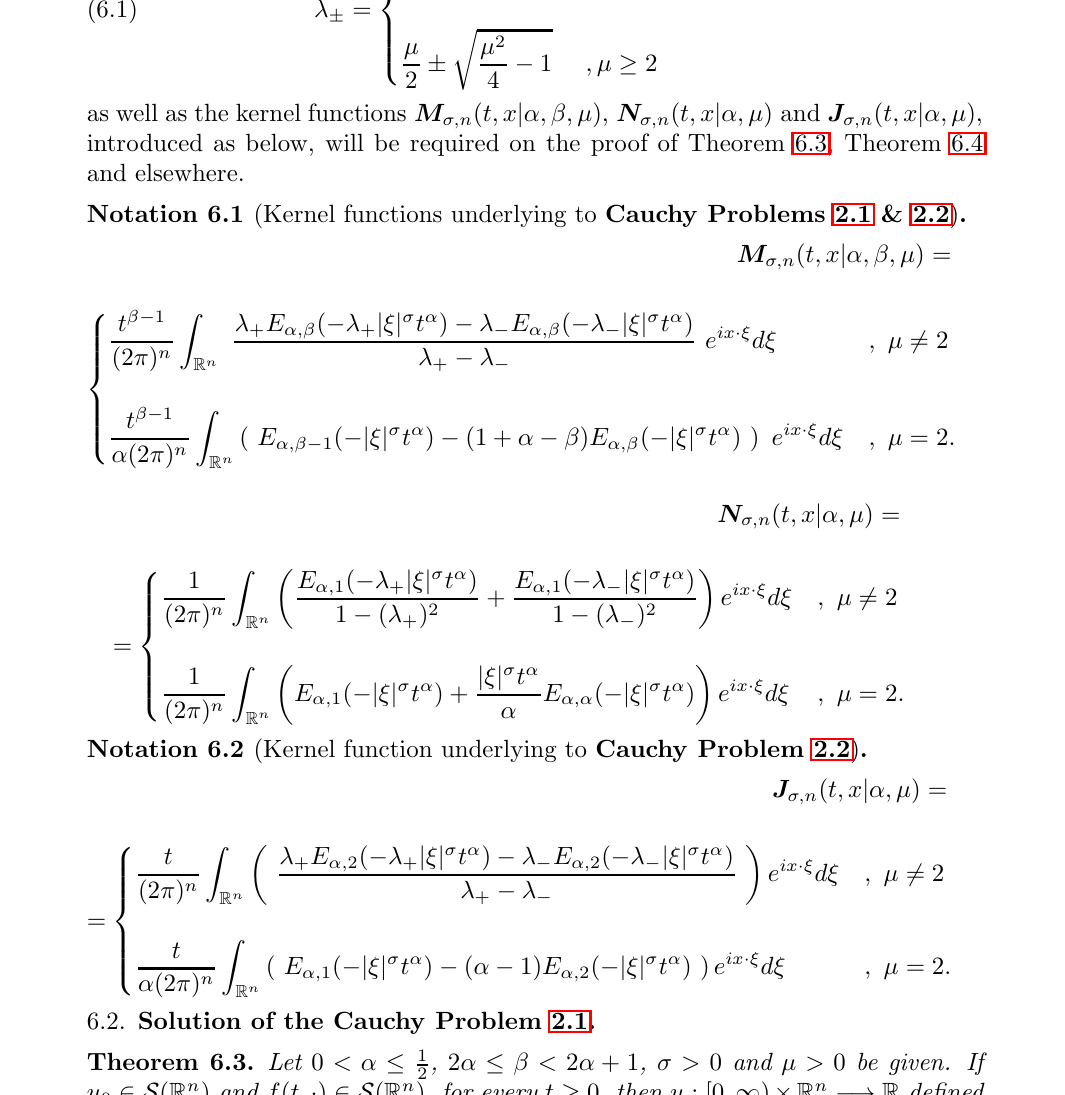
\includegraphics[width=0.70\linewidth]{figures/printed_critical_kernels_crop.png}
\caption{The critical kernels as printed on page 23.  The $M$ and $J$
lines have the erroneous signs; the $N$ line is correct.}
\end{figure}

\section{Direct counterexample to Theorem 6.4}

\begin{theorem}[Failure of the printed initial condition]\label{thm:counter}
Fix $1/2<\alpha<1$, $\sigma>0$, and $\mu=2$.  Let $u_0=f=0$ and choose
nonzero $u_1\in\mathcal S(\R^n)$ with
$\widehat u_1\in C_c^\infty(\R^n)$.  The function constructed from the
printed kernel $J_{\sigma,n}$ in Theorem 6.4 satisfies
\[
 \partial_tu(0,\cdot)=\frac{2-\alpha}{\alpha}u_1
 \ne u_1.
\]
It is therefore not a solution of Cauchy Problem 2.2.
\end{theorem}

\begin{proof}
The printed Fourier multiplier is
\[
 j_{\rm print}(t,\xi)=\frac{t}{\alpha}
 \big(E_{\alpha,1}(-z)-(\alpha-1)E_{\alpha,2}(-z)\big).
\]
Since $E_{\alpha,1}(0)=E_{\alpha,2}(0)=1$,
\[
 \frac{j_{\rm print}(t,\xi)}t
 \longrightarrow\frac{1-(\alpha-1)}\alpha
 =\frac{2-\alpha}{\alpha}.
\]
The convergence is in $C^\infty$ on the compact support of
$\widehat u_1$, by the entire power series.  Fourier inversion therefore
gives convergence in $\mathcal S$ after multiplication by
$\widehat u_1$.  Since $u(0)=0$, the asserted initial derivative follows.
The multiplier \eqref{eq:Jcorrect} instead has limit
$[1+(\alpha-1)]/\alpha=1$ and restores the datum.
\end{proof}

For the forcing kernel, the printed and correct formulas coincide only
when $\beta=\alpha+1$; equation \eqref{eq:error} gives their exact
difference otherwise.  For the velocity kernel they coincide only when
$\alpha=1$.  Thus the classical repeated-root case survives, while the
genuinely fractional critical case does not.

\section{Scope}

This correction concerns the current arXiv v2.  It refutes the critical
$\mu=2$ part of Theorem 6.4 as printed and the forced critical part of
Theorems 6.3--6.4 outside the exceptional parameter above.  It does not
claim that the paper's later dispersive or Strichartz inequalities fail:
many of those arguments use absolute-value estimates and may be insensitive
to the sign once the solution kernels are corrected.  Those downstream
claims require a separate audit.

A bounded full-source search and exact web searches found no erratum or
later correction.  Novelty is therefore provisional pending author or
specialist review.

\begin{thebibliography}{9}
\bibitem{FM}
N.~Faustino and J.~Marques,
\emph{Structurally damped $\sigma$-evolution equations with power-law
memory}, arXiv:2212.10463v2 (2023).
\end{thebibliography}

\end{document}
